\chapter{Prototype - Development and Implementation\label{cha:prototype}}
%2900
This chapter presents design and implementation of the \ep~aided environment
that provides support for \LLLs in universities.

Previous chapters (Chapter \ref{cha:litrev} and \ref{cha:systudy}) identified
recommendations and needs for successful \LLLs support. With the help of the
major stakeholders, Chapter \ref{cha:model} took these highly conceptual
requirements to the practical level of the system features. Now, in this chapter
development of these features using open-source \ep~system Mahara as a basic
platform for implementation is described.

This chapter starts with briefly discussing the overall architecture of the
environment and development toolkit. Then, each implemented component is
presented with its relation to the requested features and \LLLs recommendations
from the literature.

\section{Architecture}

Figure \ref{fig:arch} shows the overall architecture of the environment which
consists of two main components: institutionally controlled LMS and an external,
but institutionally supported \ep~system. Main implementations were carried
out in the \ep~system environment as the features prioritised by the interview
participants were largely in the \ep~domain. They included developing such
components and modules as version control, artifacts' fragments extraction,
concept mapping, timeline based progress tracking and advanced sharing options.

\begin{figure}[htp]
\centering
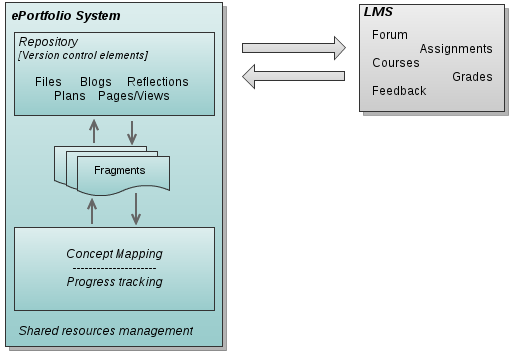
\includegraphics[width=0.8\textwidth]{CH6-F1-Architecture}
\caption{Environment architecture}
\label{fig:arch}
\end{figure}

Each component provided working functionality sufficient to demonstrate the
general concept. Non-functional requirements described in Chapter
\ref{cha:model} were not taken into account as non-essential ones in functional
prototype.

Features that involved LMS environment were not considered for implementation,
as there were enough road-map specifications discovered in the area of
\ep~development that included integration and data transfer between LMS and an
\ep~system. As well, stakeholders had not identified LMS functionality as an
important one in \LLLs context. Due to this, guidelines G1 and G6 that would
have involved LMS modifications were not supported by implementations and are
not discussed further in this section. However, LMS is still included in overall
architecture.

\section{Development Toolkit}

Using Mahara \ep~system as an initial system defined technologies that were
employed in development phase. Development and prototype systems were installed
on LAMP\footnote{\url{http://en.wikipedia.org/wiki/LAMP_(software_bundle)}}
software bundle for Linux which included Apache HTTP Server, MySQL database
server and PHP. These were the basic components for building a general purpose
web server.

Development environment consisted of the
Eclipse\footnote{\url{http://www.eclipse.org}} Platform with PHP Development
Tools\footnote{\url{http://eclipse.org/pdt}}.

Following standards and external packages were used during implementation:

\begin{itemize}

\item HTML5 + CSS -- standards combined with JavaScript used for drawing
diagrams that represent concept maps, developing a dynamic timeline and
accessing fragments of media (audio/video);

\item jQuery\footnote{\url{http://jquery.com}} -- a JavaScript library that
simplifies HTML document traversing, event handling, animating, and Ajax
interactions for rapid web development;

\item jQuery UI\footnote{\url{http://jqueryui.com}} -- a JavaScript library
built on top of the jQuery for development of highly interactive web applications;

\item jCrop v0.9.9\footnote{\url{http://deepliquid.com/content/Jcrop.html}}
-- jQuery Image Cropping Plugin used in artifacts fragments (Section
\ref{sec:frag});

\item Graphic JavaScript Tree with
Layout\footnote{\url{http://www.codeproject.com/KB/scripting/graphic_javascript_tree.aspx}}
-- a library that allows drawing dynamic concept maps. This library was
significantly modified to meet the needs of the project.
\end{itemize}

Prototype functionality was tested mainly in Google
Chrome\footnote{\url{http://www.google.com/chrome}} v14.0 and Mozilla
Firefox\footnote{\url{http://www.firefox.com}} v4.0 web browsers. Other web
browsers (e.g. Microsoft Internet
Explorer\footnote{\url{http://www.microsoft.com}}) that did not provide native
support for HTML5 elements such as Canvas, required for concept map layout, and
embedded video/audio, used in artifact's fragments, were not used in testing.

\section{Implementations}

Components added to the standard Mahara \ep~installation were expected to
address the requirements developed by the stakeholders and derived from the
literature review. In most cases, the stakeholders provided their own vision of
what kind of features could have been implemented to solve particular problems.
Their suggestions were used during development. In some cases when the
stakeholders could not propose any suitable solution, it was necessary to refer
to other domains and analyse solution to similar problems. Most suitable, as
well as feasible for development, approach was implemented.

Table \ref{tab:implement} matches implemented components to the guidelines they
support and the requested features. Guidelines and features identifiers used in
this table were described in Sections \ref{sec:needs} and \ref{sec:elicit},
respectively.

\begin{center} \small
    \tablefirsthead{
     \hline
     \multicolumn{1}{|c||}{} &
     \multicolumn{5}{c|}{\textbf{Implemented components}} \\ \cline{2-6}}
    \tablehead{
     \hline
     \multicolumn{6}{|l|}{\small\sl continued from previous page}\\
     \hline
     \multicolumn{1}{|c||}{} &
     \multicolumn{5}{c|}{\textbf{Implemented components}} \\  \hline} 
    \tabletail{
     \hline
     \multicolumn{6}{|r|}{\small\sl continued on next page}\\ \hline}
    \tablelasttail{\hline} 
	\bottomcaption{Implemented \ep~system components}
    \begin{supertabular}{| c || p{2cm} | p{2cm} | p{2cm} | p{2cm} | p{2cm} |}
     \textbf{Guidelines} & 
     \textit{Version \newline control \newline Section \ref{sec:version}} & 
     \textit{Concept mapping \newline Section \ref{sec:mapping}} & 
     \textit{Artifacts' fragments \newline Section \ref{sec:frag}} & 
     \textit{Progress tracking \newline Section \ref{sec:timeline}} & 
     \textit{Advanced \newline sharing \newline Section \ref{sec:sharing}} \\
     \hline \hline
     \rowcolor[gray]{.8} G1 & & & & & \\ \hline
     G2 & I3 & & & C1 & B3\\ \hline
     G3 & I3 & & & & B3 \\ \hline
     G4 & & K1, K2 & K2 & & \\ \hline
     G5 & C2, C3, C4 & & C4 & & C5, C6 \\ \hline
     \rowcolor[gray]{.8} G6 & & & & & \\ \hline
     G7 & & P1 & & P1, P2, P3 & \\ \hline
     G8 & & A1, A2, A3, \newline A4, A5, A6 & & & \\ \hline
     G9 & & B1 & K3 & P4, P5 & \\ \hline
    \end{supertabular}
    \label{tab:implement}
\end{center}

Table \ref{tab:implement} also shows that, as it has been initially planned,
implementations are covering at least partially each of the guidelines. Formal
requirements for each component are described in the relevant sections of
Appendix \ref{app:specification}. Detailed screenshots of the interface can be
found in Appendix \ref{cha:appscreen}.

\subsection{Version Control Elements}
\label{sec:version}
Implementing this feature was very straightforward compared to other features.
Suggested by the stakeholders functionality of having versions of the shareable
resources was easy to fit into \ep~system. Versioning was implemented in a
simple way that allowed only \textit{parent} $\to$ \textit{child} relationship
between versions and did not support versions branching as in complex revision
control systems. As well, this component does not perform an automated
difference analysis between versions because pages can incorporate both textual
and block elements that would make it technically difficult and time consuming to
implement this kind of analysis. Therefore, analysing the difference between
versions was left for users.
 
As can be seen from Table \ref{tab:req1}, this feature was implemented only for
\ep~pages. It was considered sufficient to demonstrate the general concept as
\ep~pages could be shared with others and experience of using this feature can
be easily transferred to other shareable resources.

Adopting version control elements in \ep~system was expected to provide support
for communication and feedback-response cycle between students and lecturers, as
well as between students and audience outside of institutional environment.

\subsection{Concept Mapping Module}
\label{sec:mapping}
Addressing the challenges of \ep~knowledge management\footnote{In this thesis,
the \ep~knowledge management is referred to in terms of creating knowledge,
sharing it, managing and organizing it in \ep~space.} and development of
graduate attributes, that represent the core learning outcomes, skills and
qualities that students should develop during their university education, as
have for example been outlined in \citet{Hughes2010}, was a complex problem
which required a creative approach and no clearly suggested solution from the
stakeholders. While looking at the other areas for potential solution, it was
discovered that qualitative data analysis and knowledge visualization using
concept mapping tool have properties suitable for \ep~domain. Like \ep~work,
qualitative data analysis is characterised by rich data sets, opening the
possibility of borrowing well established techniques. Concept maps had potential
as a supporting tool for organizing these data sets into concepts and
visualising them in a way that could be understood by relevant audiences.

This section describes how bringing these two techniques together helped to
develop a solution for the problems outlined earlier.

\subsubsection{Parallels to qualitative research}

An \ep~can be called a container that needs to be organized, with students not
always knowing which items to select and where the items they put in their
\ep~should go. Students start their \ep~work by collecting \textit{raw} data
available from formal learning and outside activities and transforming it into
information that they decide to put into their \ep. After working with and
reflecting on this information students arrive at knowledge. A parallel with
qualitative data analysis can be drawn here where researchers either develop new
theories from data, moving from specific observations to general concepts and
theories (inductive approach), or they try to check if their data map against
the theories that are already known and understood (deductive approach)
\citep{Strauss2008,Patton2002}. An assumption here is that analyzing one's own
learning process takes similar steps as qualitative data analysis: small bits,
specific data that learners are collecting, contribute to the bigger picture of
knowledge development. The difference is that the learner developing their
\ep~is not aware of the existing theories yet. These theories are the concept
structures that exist in the understanding of society, institution and
employers. However, these must be eventually understood and \textit{made their
own} by the learner. Like the qualitative researcher, the learner needs to
immerse themselves in their data and to come to an understanding of the kind of
material they should be collecting in their \ep~and the concepts that express
their learning goals. They need to find (and to a certain degree construct by
exposing themselves to learning opportunities) evidence in their data to show
that they conform to these concepts.

In qualitative research, a number of techniques are available to the researcher
in managing, analyzing and interpreting their data, such as coding, grouping,
generating categories and themes, rearranging and sorting \citep{Marshall2010}.
To support these techniques, specialized qualitative data analysis software
(QDAS), like
NVivo\footnote{\url{http://www.qsrinternational.com/products_nvivo.aspx }} and
MAXQDA\footnote{\url{http://www.maxqda.com}}, has been developed which largely
allows coding, linking and mapping unstructured information. Although, QDAS
could provide students with necessary functionality for data analysis, it cannot
substitute the role of an \ep~system in the learning process. Reasons for
that are outlined in Table \ref{tab:qdas}.

\begin{table}[htb]
  \begin{center}
    \begin{tabular}{| p{6cm} | p{6cm} |}
    \hline
     \multicolumn{1}{|c|}{\textbf{QDAS}} &
     \multicolumn{1}{c|}{\textbf{\ep~system}} \\
     \hline
     Help researchers to understand data & Help students to understand data and
     theories \\ \hline 
     Develop codes, concepts and theories; visualize relations between concepts
     & Showcase students' growing understanding of theories and their data \\
     \hline 
     Produce a report as an end point of the research  & Does not have an end
     point; data is constantly evolving; old concepts are changing and new are
     emerging with changing understanding of these concepts \\ \hline 
    \end{tabular}
  \end{center}
  \caption{Conceptual difference between QDAS and \ep~system}
  \label{tab:qdas}
\end{table}

However, the strength of QDAS is in how it allows to work closely with data.
Researchers \textit{label} data with codes, not just in order to connect these
labels later, but as an opportunity to \textit{dive} into their data by
re-reading, listening or watching it over and over again. This strength is
important for students as they need to revisit their material as their
understanding of concepts grows.

Currently, the majority of \ep~systems allow tagging their content with
user-defined tags. However, according to the results of interviews with
students, tagging does not provide necessary meaning to the \ep~data,
cannot show relations between concepts and does not allow building a flexible
structure. To address this problem, concept mapping was introduced into
\ep~environment to help students to be able use the same techniques available in
qualitative data analysis to manage unstructured data and develop learning
concepts in their \ep.

\subsubsection{Concept maps}

\citet{Mcaleese1998} formally defines a concept map as a directed acyclic graph
that consists of a set of Concept Labels and a non-empty set of Relationships
between Concepts. Putting it simply, concept maps are graphical representation
of the hierarchy of knowledge concepts and connections between them
\citep{Novak2008}.

Concept maps fit well with the qualitative data analysis techniques, outlined in
the previous section, as they are dynamic, process-oriented and give learners an
opportunity to engage in the learning process \citep{Mcaleese1998} which is
important for \LLLs \citep{Schuetze2006,Divjak2004}. Maps are created over time
by the learner who is engaged in a process of reflection, collecting and
selecting appropriate examples of their work. With concept maps learners can
interpret their personal knowledge and map this knowledge and individual
examples against the existing theories. The hierarchical nature of the concept
map allows for organizing concepts from the high level abstract concept to the
more specific concepts. This property can be used by students for managing and
structuring data in their \ep s. In addition, while describing future directions
for \ep~technology, Cambridge \citeyearpar{Cambridge2010} suggested that
visualization in the form of concept maps could be a potential way of generating
reflections.

QDAS already offers tools similar to concept maps in form of textual hierarchies
of nodes/terms/labels/concepts or as diagrams that show relations between
labels. Adding concept maps functionality to an \ep~system might make it
possible to borrow well established techniques of qualitative data analysis and
help students, who are analyzing their learning, to formally do what QDAS
already does informally. 

Concept maps have been already successfully used to in education to communicate
complex ideas, assess understanding of learning objectives, elicit knowledge and
provide conceptual frame for learning \citep{Novak2010}. A complete review of
the concept maps is beyond the scope of this thesis. For detailed examples and
evaluation of effectiveness of this tool refer to The Institute for Human and
Machine Cognition research group report \citep{Canas2003}.

\subsubsection{Component implementation}

The framework (Figure \ref{fig:mapping}), presented in this section, adopts the
idea of concept maps in terms of developing or understanding concepts and
relations between them. Following qualitative data analysis techniques, students
create their own codes for the concepts which later form a concept map. Students
can also be provided with a map structure predefined by universities as a set of
Graduate Attributes in form of abstract concepts. Going thought the program of
study, students can learn to understand these concepts and recognize the
valuable examples of their work in the learning process.

\begin{figure}[htb]
\centering
\includegraphics[width=1\textwidth]{CH5-F2-Mapping}
\caption{Object Role Modeling (ORM) diagram of the concept map structure}
\label{fig:mapping} 
\end{figure}

Each map can have an abstract core or key concept and optional supporting
sub-concepts. In this framework, students can provide definitions for the
concepts, which gives them descriptions from their point of view. Examples
chosen by students for these definitions are parts of the items (Section
\ref{sec:frag}), or entire items, from the \ep~repository which represent their
personal experience and achievements. Each example has to be supported by the
student's reflection that should explain what is special about this example, or
how it addresses this specific concept. It is expected to help students
understand that their ePortfolio space is not a place for ``dumping'' all
possible items. Each element of an ePortfolio is an important example of their
personal and professional development carefully selected to demonstrate learning
progress.

An \ep~concepts structure can be represented as shown in Figure \ref{fig:mapex}.
Data for the example was taken from the examples offered by \citet{Marzano1993}
on how to assess \LLLs standards.
 
\begin{figure}[htb]
\centering
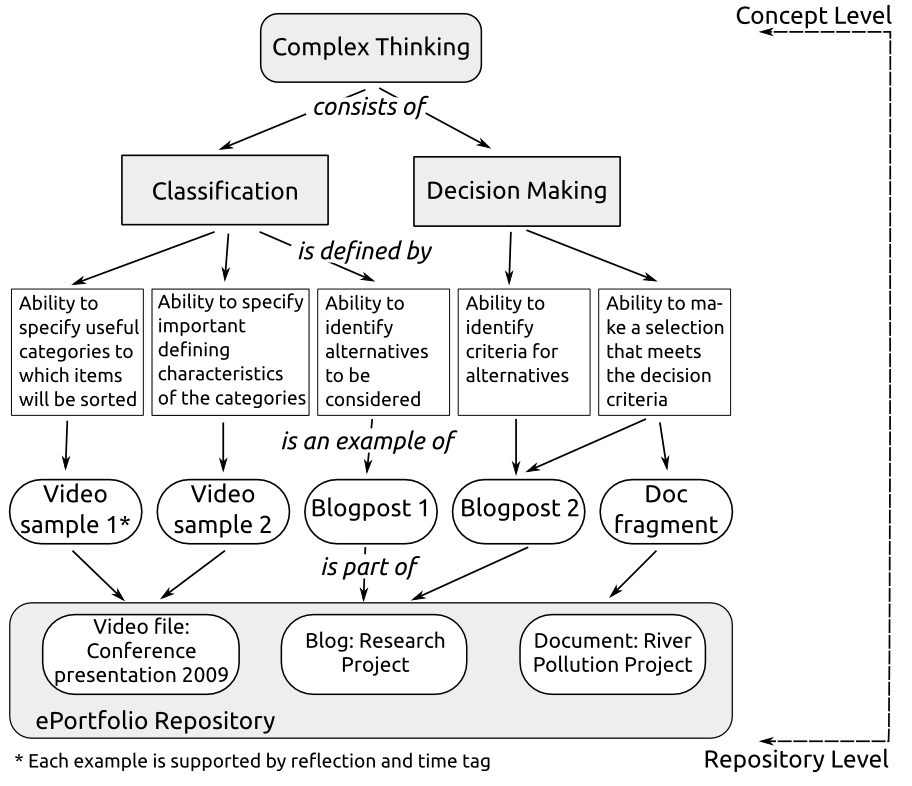
\includegraphics[height=0.5\textheight]{CH5-F3-Map-Example}
\caption{Concept mapping framework applied to the example}
\label{fig:mapex} 
\end{figure}

Due to the dynamic nature of learning process this kind of structure might never
be complete. It is constantly changing as students deepen their understanding
and potentially find more suitable evidence to underpin their development.

The expectations were that this approach would allow students to:

\begin{itemize}
  \item Manage and structure large amounts of information in their \ep:
  students will be able to organize and navigate through the information, find
  relations between the content and the concepts and see the data in their
  \ep~from various perspectives: from an item belonging to different
  structures; from a concept containing multiple evidences; and from items and
  concepts attached to a timeline (Section \ref{sec:timeline});

\item Share their progress/development map with others for feedback or
evaluation: students will be able to create specific structures for various
purposes to show to the audience specific parts of their \ep~(for example,
share with a potential employer communication and writing skills developed over
the last year at university);

\item Access and address institutional graduate attributes: by providing
students with a concept map of the graduate attributes (maybe even already
supported by the institutional definitions), universities would be able to
help students to understand the skills requirements of their study area and look
at their study program from the \LLLs perspective;

\item Develop a flexible structure for self-directed learning: students are
provided with all operations necessary to make their structures flexible such as
creating new concepts, removing or merging existing ones, creating links between
structure fragments and taking snippets of \ep~items as examples (Section
\ref{sec:frag});

\item Facilitate setting up learning/development goals and expressing students
visions of their knowledge: constructing their own concepts and definitions
might encourage students to think of what skills are important to them, how they
understand these skills and how it links to their learning outcomes.
\end{itemize}

\subsection{Artifacts' Fragments Extraction}
\label{sec:frag}

Artefact's fragments extraction was developed as a part of concept mapping
module. This feature allows selecting of any artifact's fragment and using
it as an example in definitions of the concepts described in the previous
section. Using fragments or parts of artifacts could be useful for a number of
reasons: it allows the presentation of different parts of artifacts to different
audiences, but at the same time avoiding files duplication; it saves user's time
that would be spent on cropping images or videos; it .

To demonstrate this feature, the following artifact fragments were implemented:

\begin{itemize}
  \item Image:
  \item Video:
  \item Text:
  \item Blog:
  \item Bookmark:
\end{itemize} 

Files that do not support fragments extraction allow attaching an entire
artefact


From the perspective of this component evolving Media Fragments 1.0
specification \citep{MediaGroup2011} becomes very useful as it describes the
ways of extracting temporal and spatial media fragments using Uniform Resource
Identifiers (URI). Once it is finished, this specification could be adopted in
the \ep~system for improved fragments description and extraction.

\subsection{Learning Progress Tracking}
\label{sec:timeline}

In addition, custom time tags were included within this structure that allowed
any map to be transformed into a timeline. This was identified as a requirement
by students as a way to facilitate the tracking of their personal progress.
Students will be able to define their own time frames and organize their maps
according to their needs. Looking at the information from different perspective
allows seeing progress over time and may lead to the better understanding of
one's personal development. It can also help to showcase the progress for
evaluation or share it with others for feedback purpose.



To sum up, this conponent is expected to support tracking personal progress in
various areas and aspects. Generating timelines could add a temporal dimension
to students progress analysis: they would be able to see how their skills evidence
changed in time, how feedback received from the others reflects their growing
understanding, what achievements they have made and what concepts require more
input;


\subsection{Advanced Sharing Options}
\label{sec:sharing}
What was added: history, re-share, notifications, share by email.


\section{Prototype Iterations and User Tests}
 
Before formal evaluation was undertaken, implemented functionality had been
tested by users. Overall, time and resources constraints of the project allowed
for two planned prototype iterations. Each iteration produced a workable version
of the implemented features. At the end of each iteration, the functional
prototype was presented to a student and a lecturer selected from the
participants of the requirements elicitation phase who had agreed to continue
their participation in this research.

Each feedback session included up to an hour demonstration and discussion of the
implemented functionality. Users were encouraged to give their ideas about
potential improvements and 

Feedback between iterations was very useful as it provided information on
necessary improvements and drawbacks of current implementations. Users were
generally satisfied with the improvements and made largely positive comments.
However, several issues were noted: \ldots

All discovered issues were addressed in the later versions of the prototype
in preparation for the formal evaluation stage.

\section{Summary}

This chapter presented \ldots